\documentclass{article}
\usepackage{graphicx}
\usepackage{geometry}

\geometry{
  letterpaper,
  total={8.5in,11in},
  left=0mm,
  right=0mm,
  top=0mm,
  bottom=0mm,
  noheadfoot
}

\pagestyle{empty}

\begin{document}

\newgeometry{
  letterpaper,
  total={8.5in,11in},
  left=0mm,
  right=0mm,
  top=0mm,
  bottom=0mm,
  noheadfoot
}

\begin{figure}[p]
  \centering
  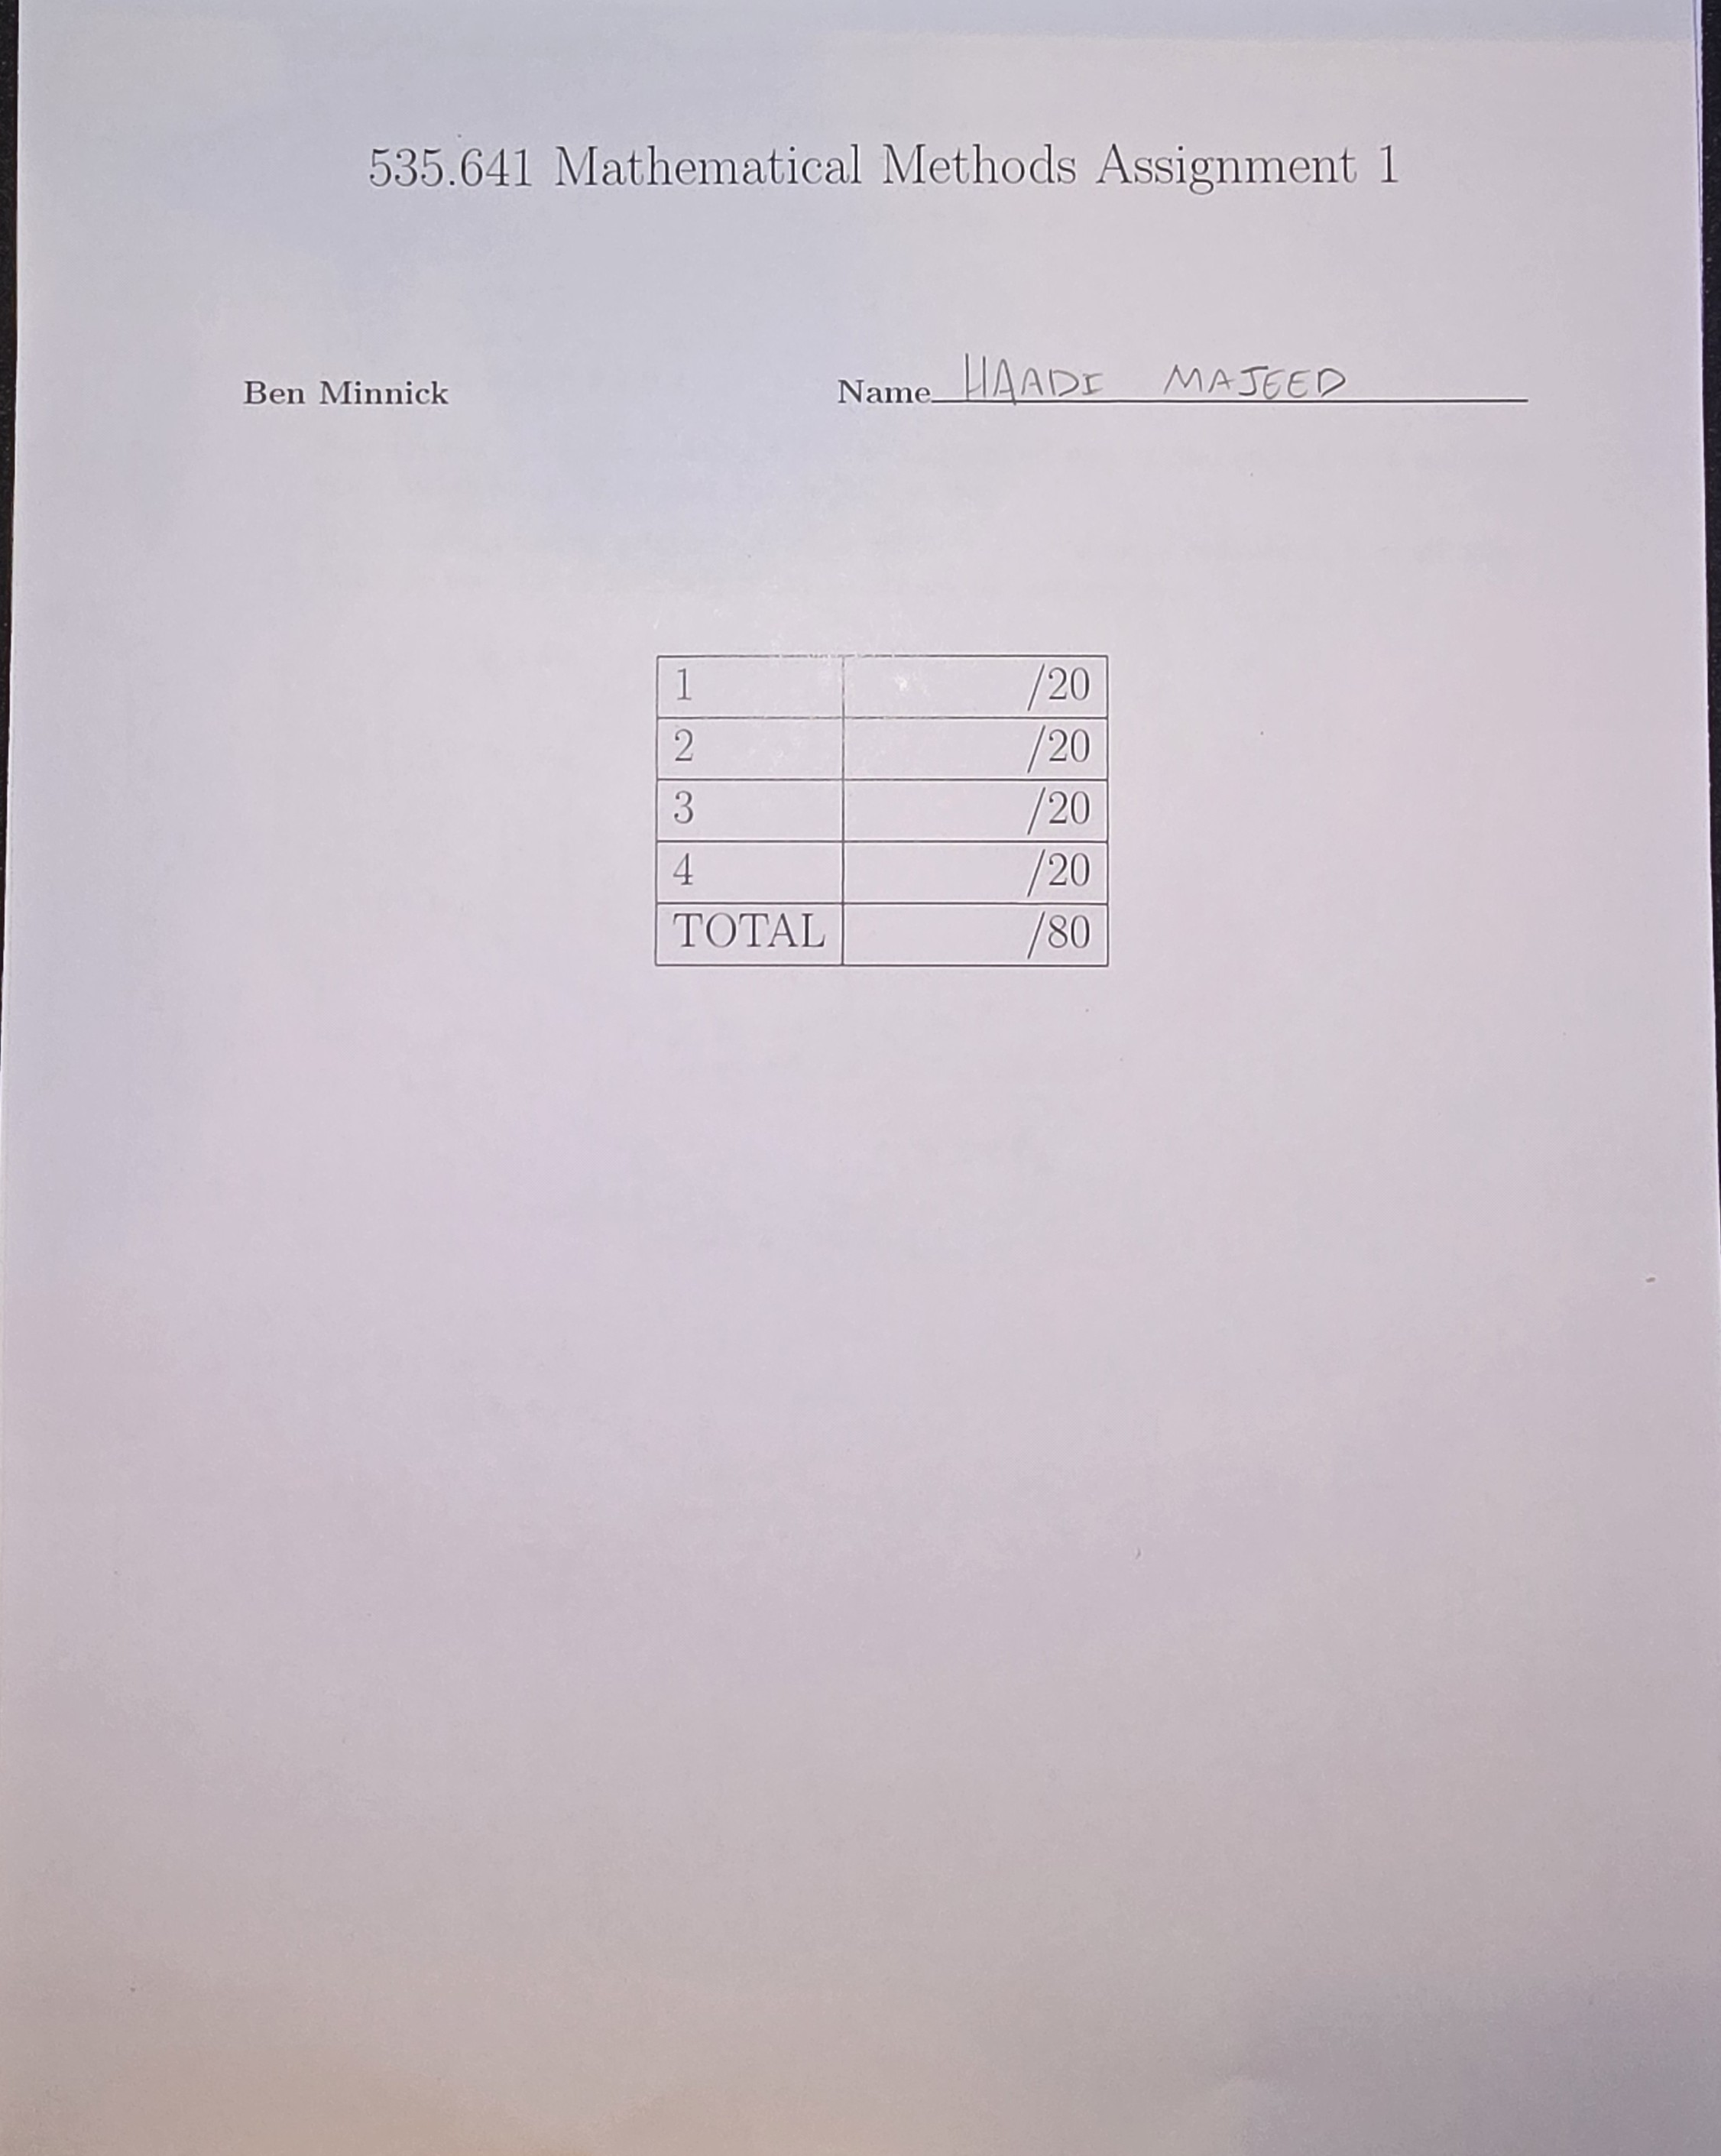
\includegraphics[width=\paperwidth,height=\paperheight,keepaspectratio,angle=0]{page1.jpg}
\end{figure}

\clearpage

\begin{figure}[p]
  \centering
  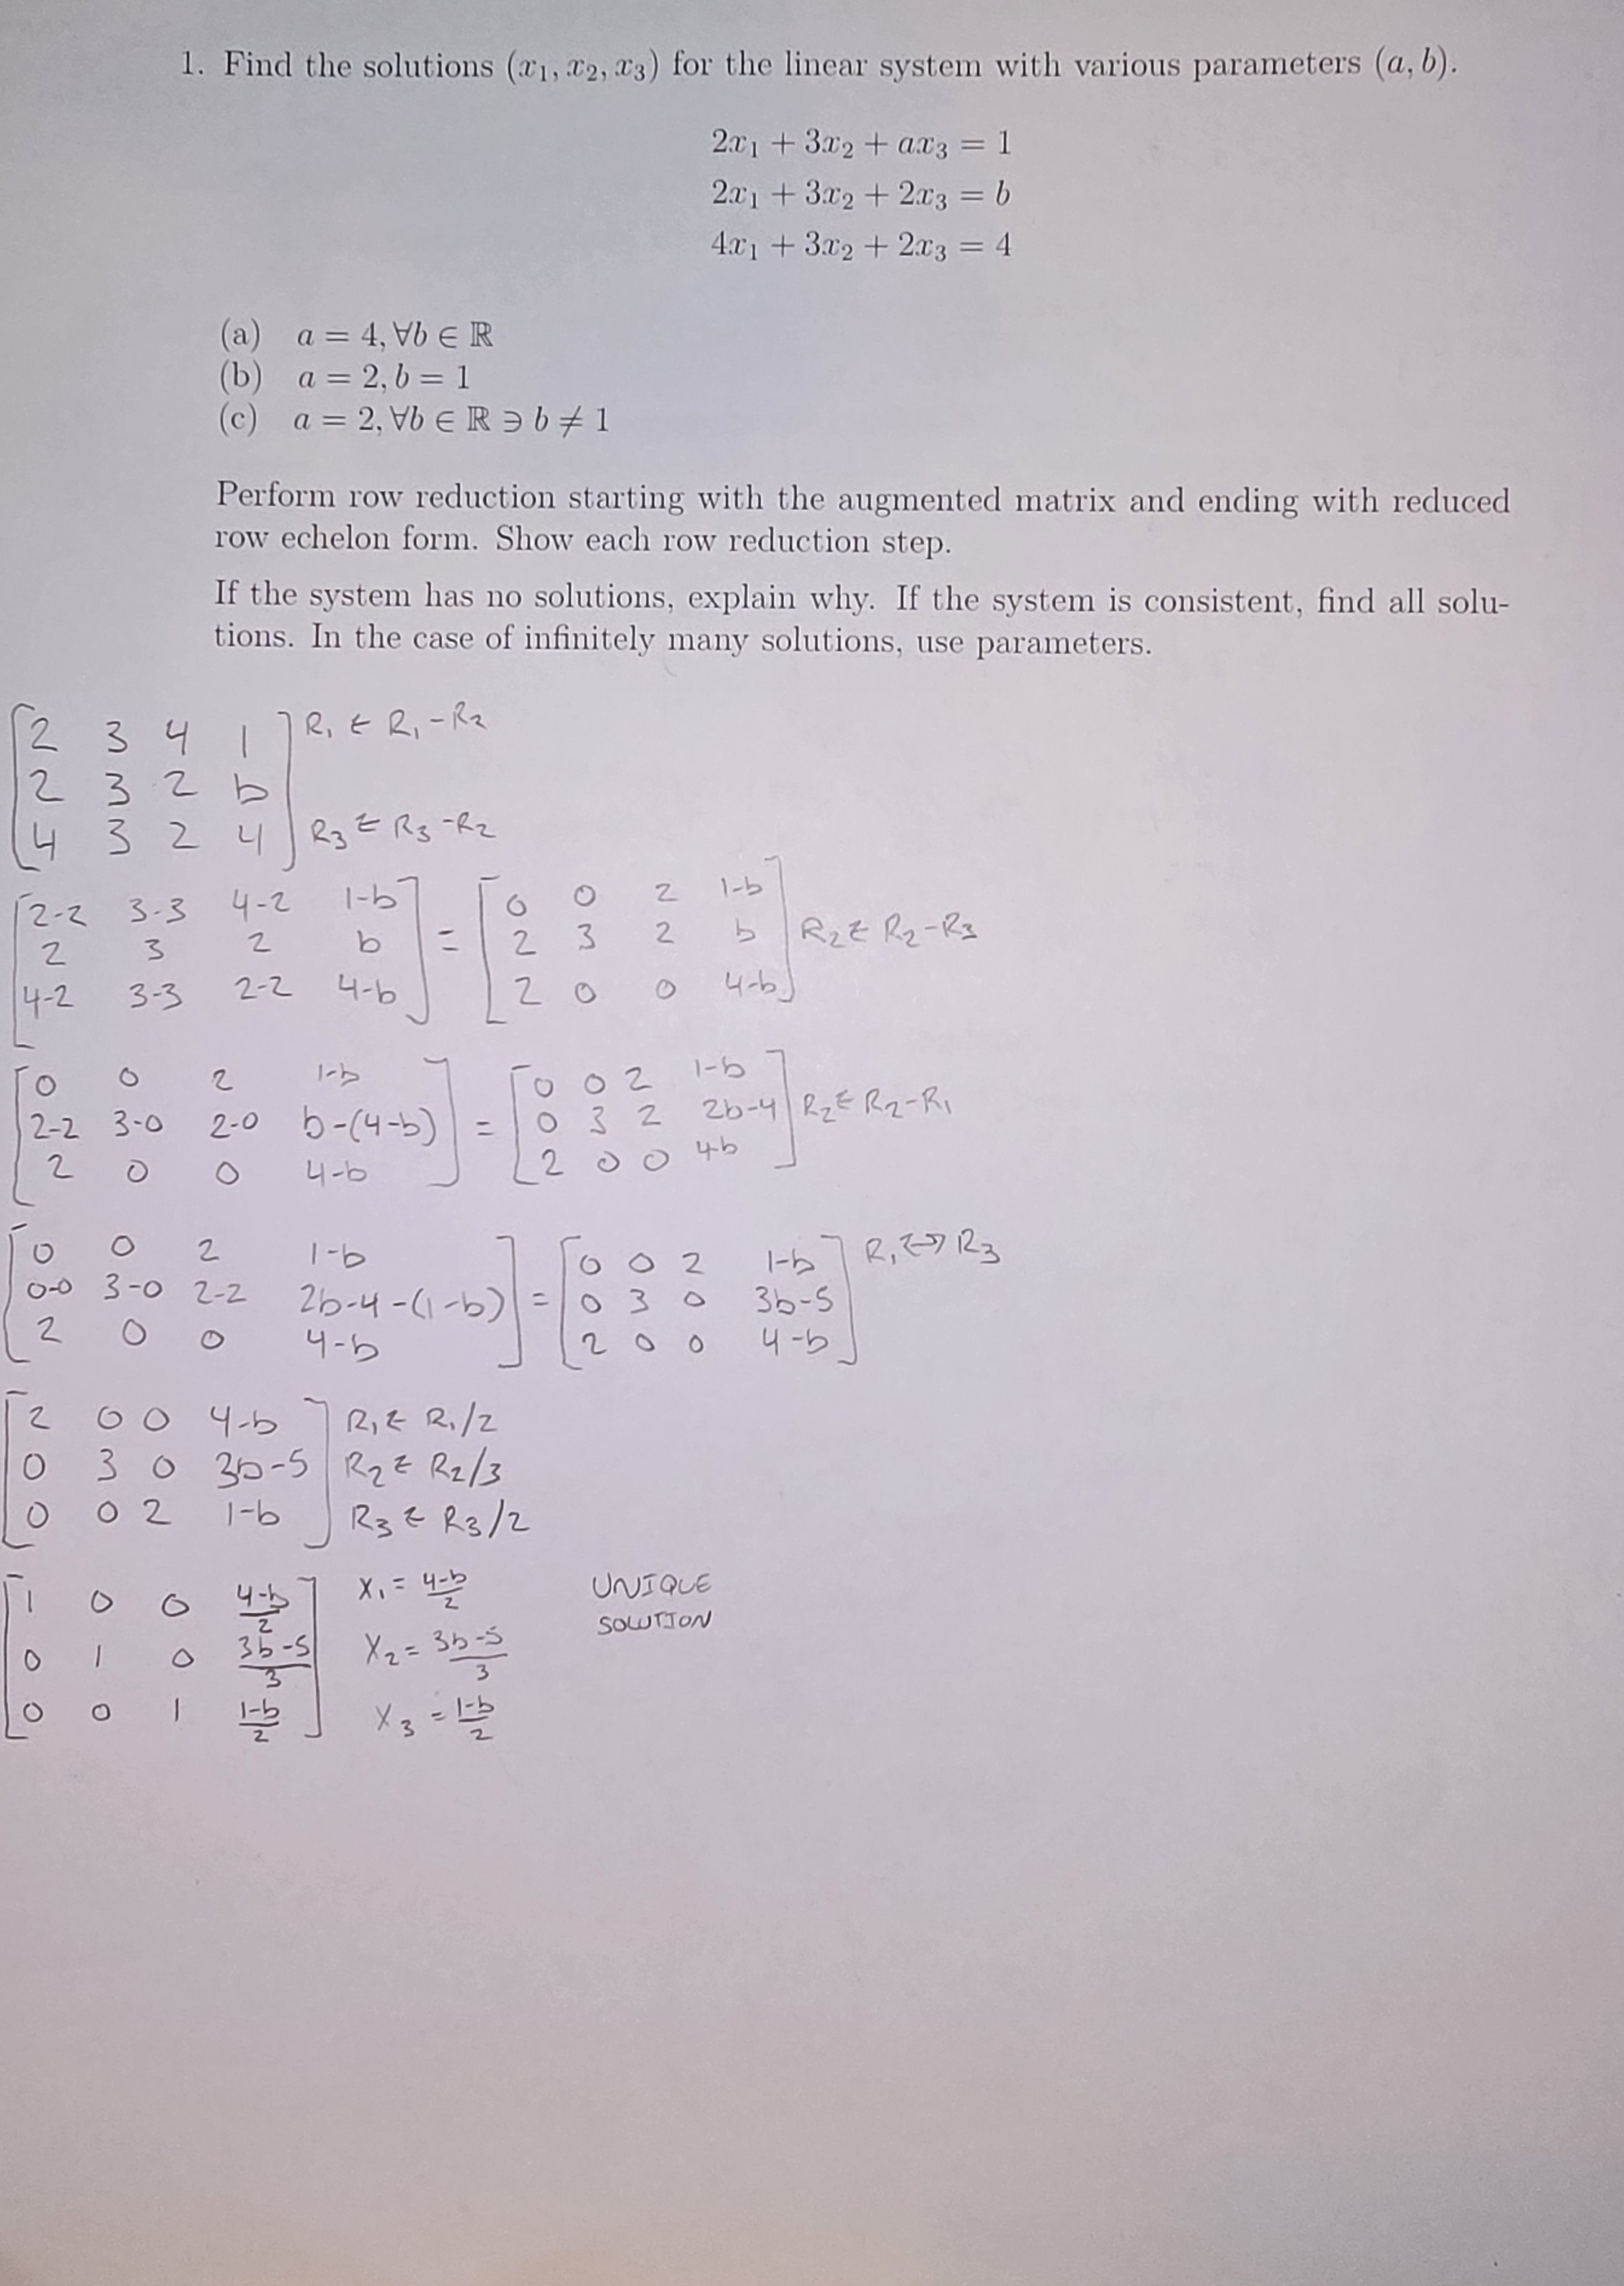
\includegraphics[width=\paperwidth,height=\paperheight,keepaspectratio,angle=0]{page2.jpg}
\end{figure}

\clearpage

\begin{figure}[p]
  \centering
  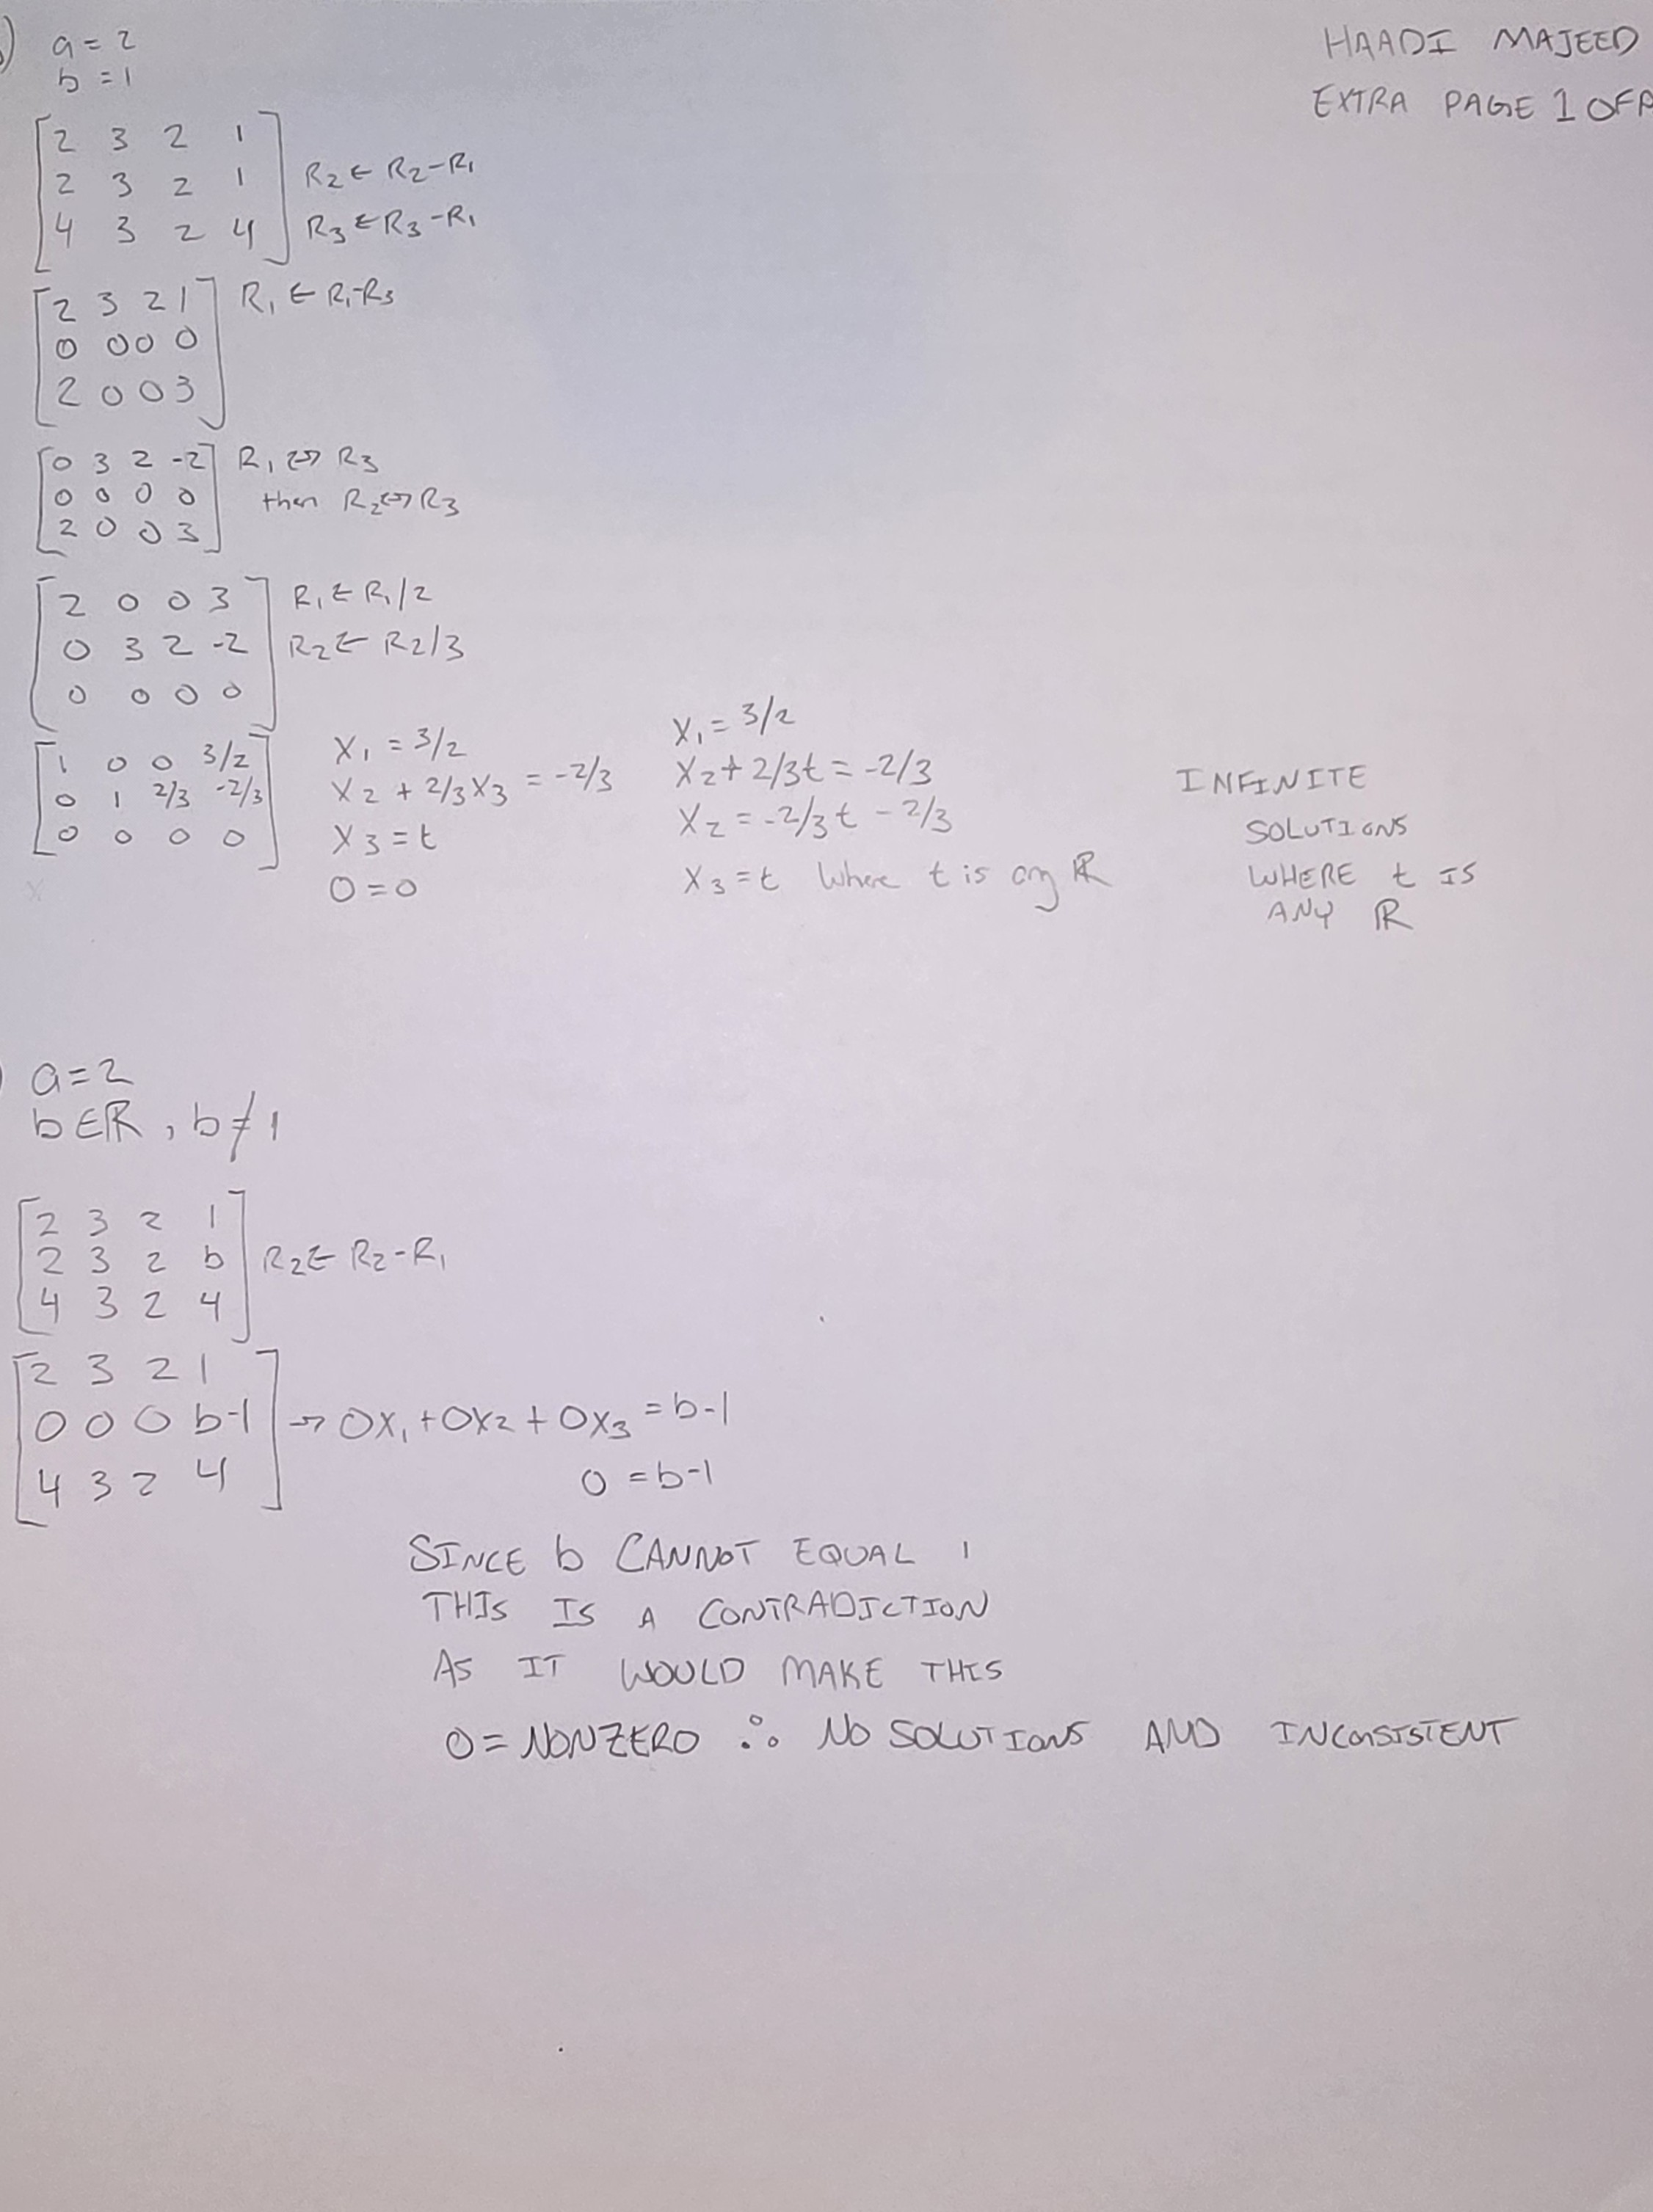
\includegraphics[width=\paperwidth,height=\paperheight,keepaspectratio,angle=0]{page3.jpg}
\end{figure}

\clearpage

\begin{figure}[p]
  \centering
  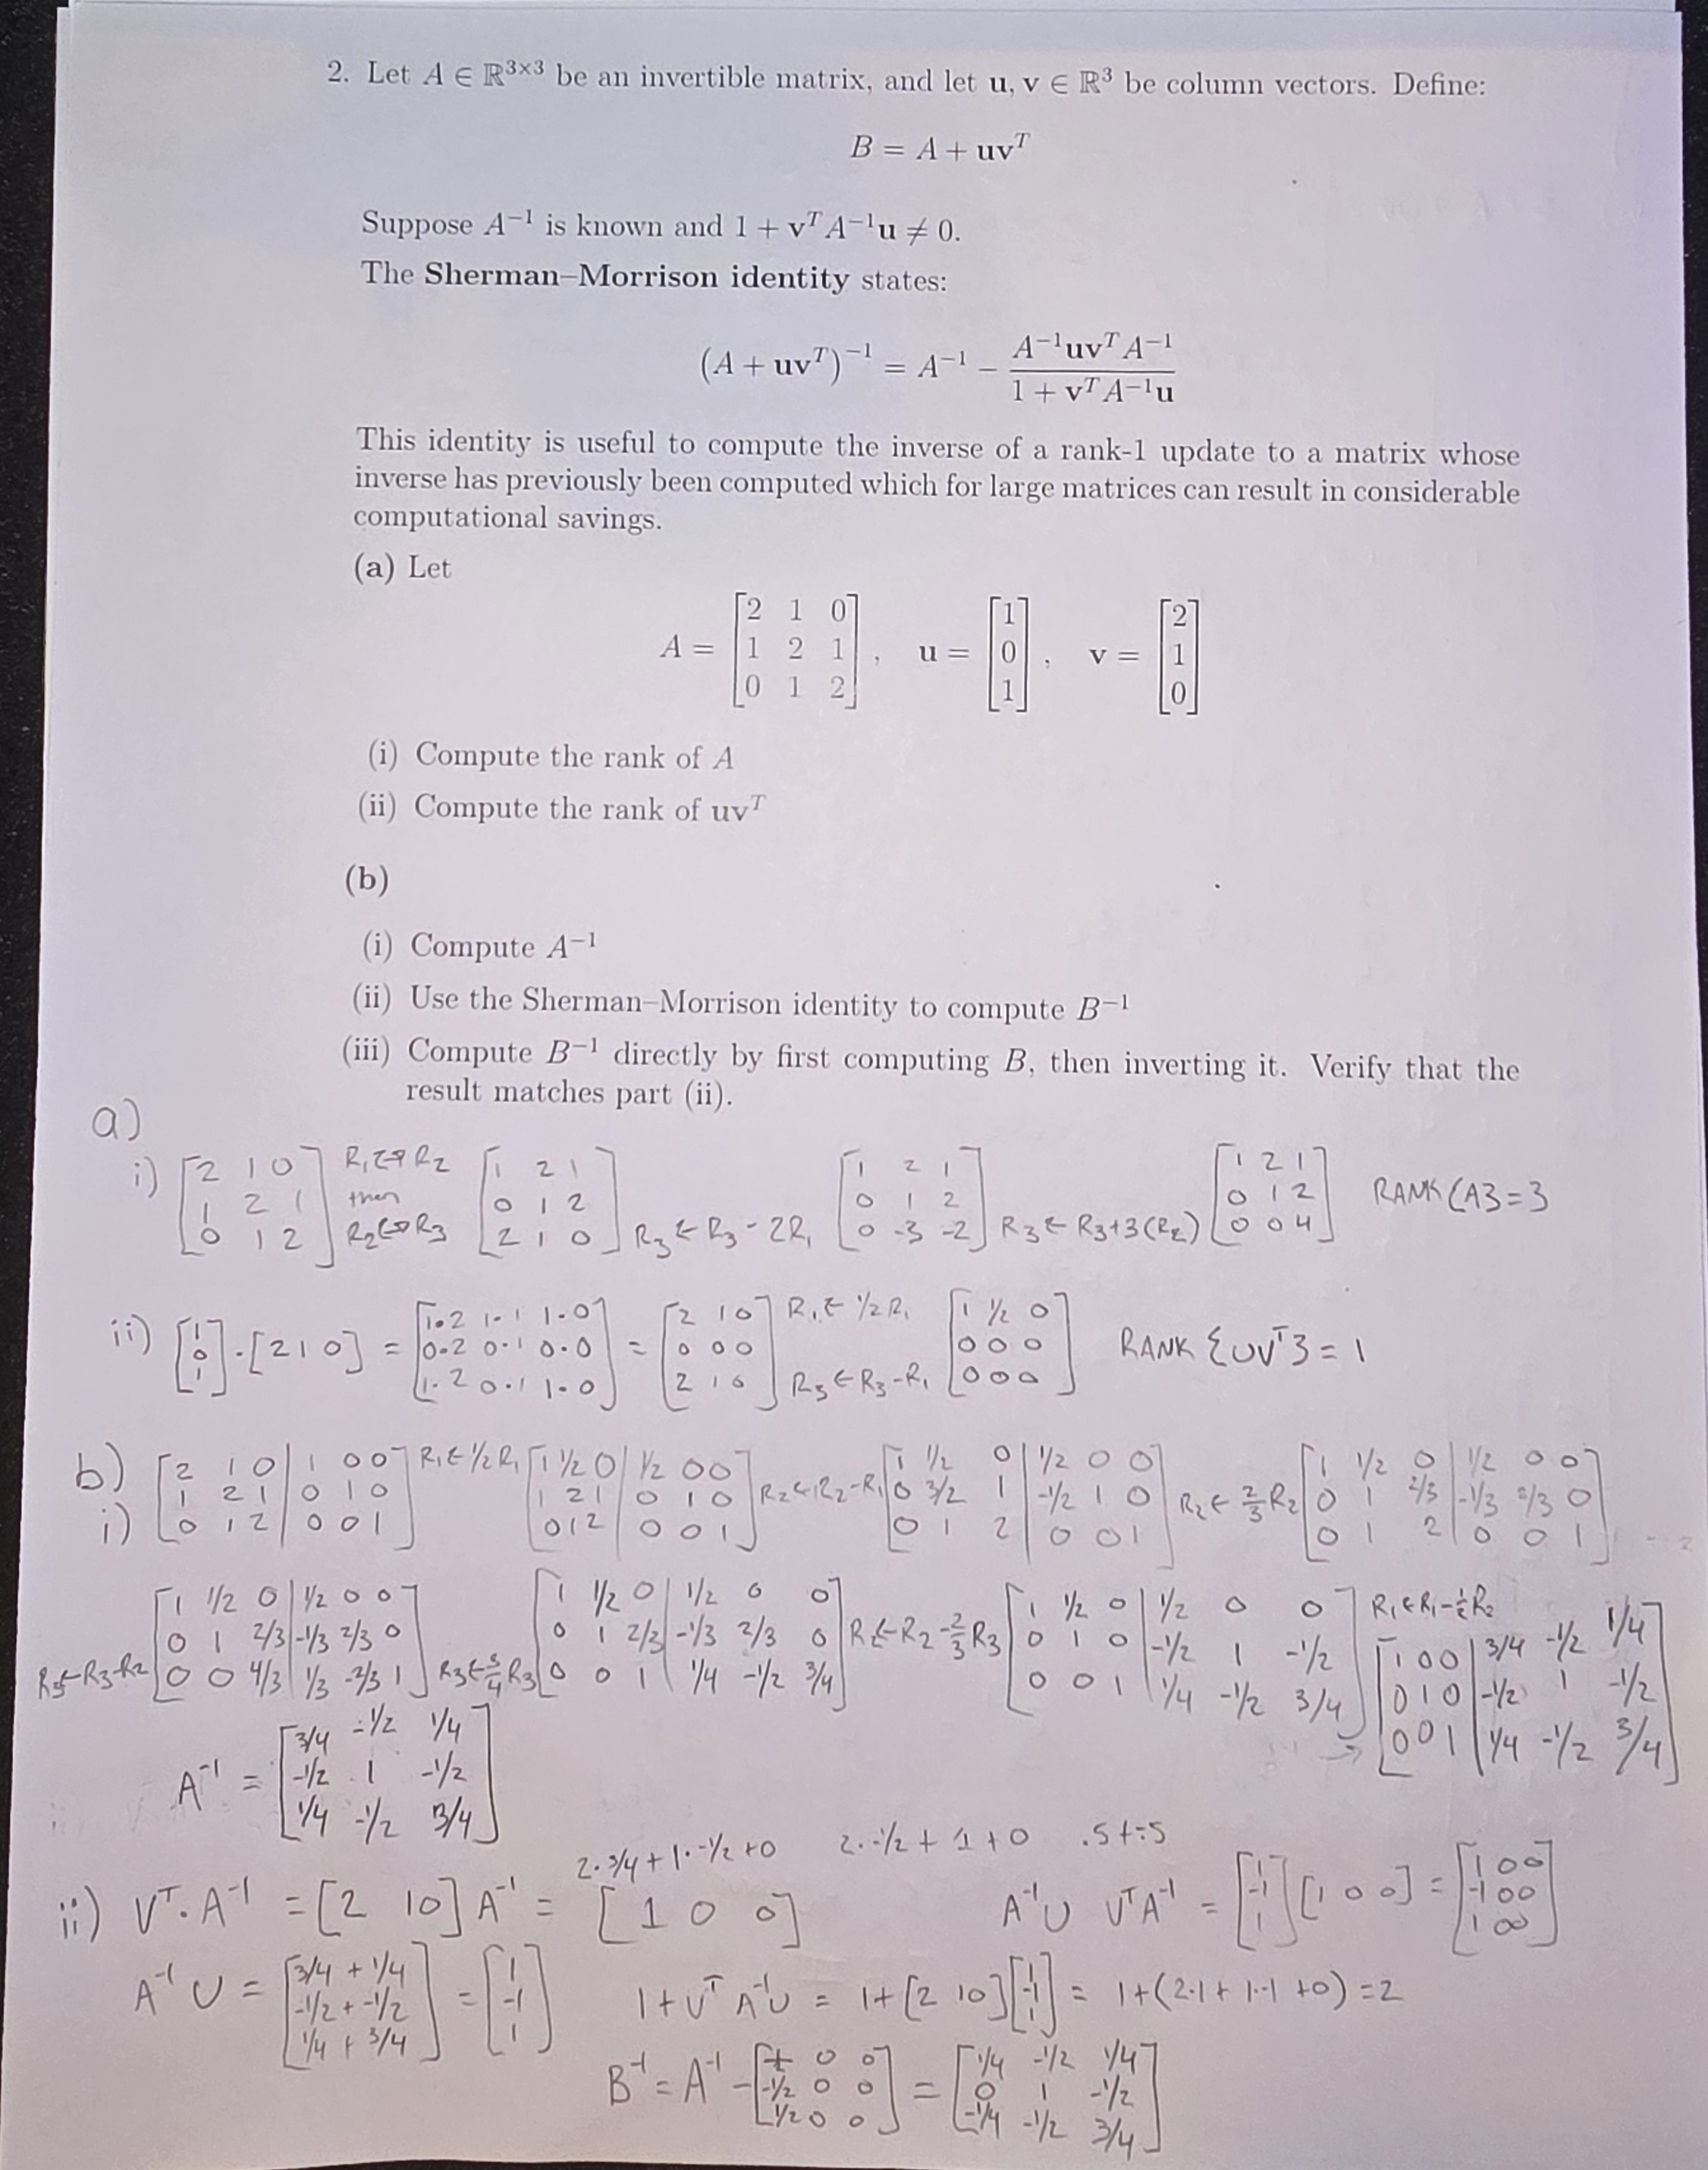
\includegraphics[width=\paperwidth,height=\paperheight,keepaspectratio,angle=0]{page4.jpg}
\end{figure}

\clearpage

\begin{figure}[p]
  \centering
  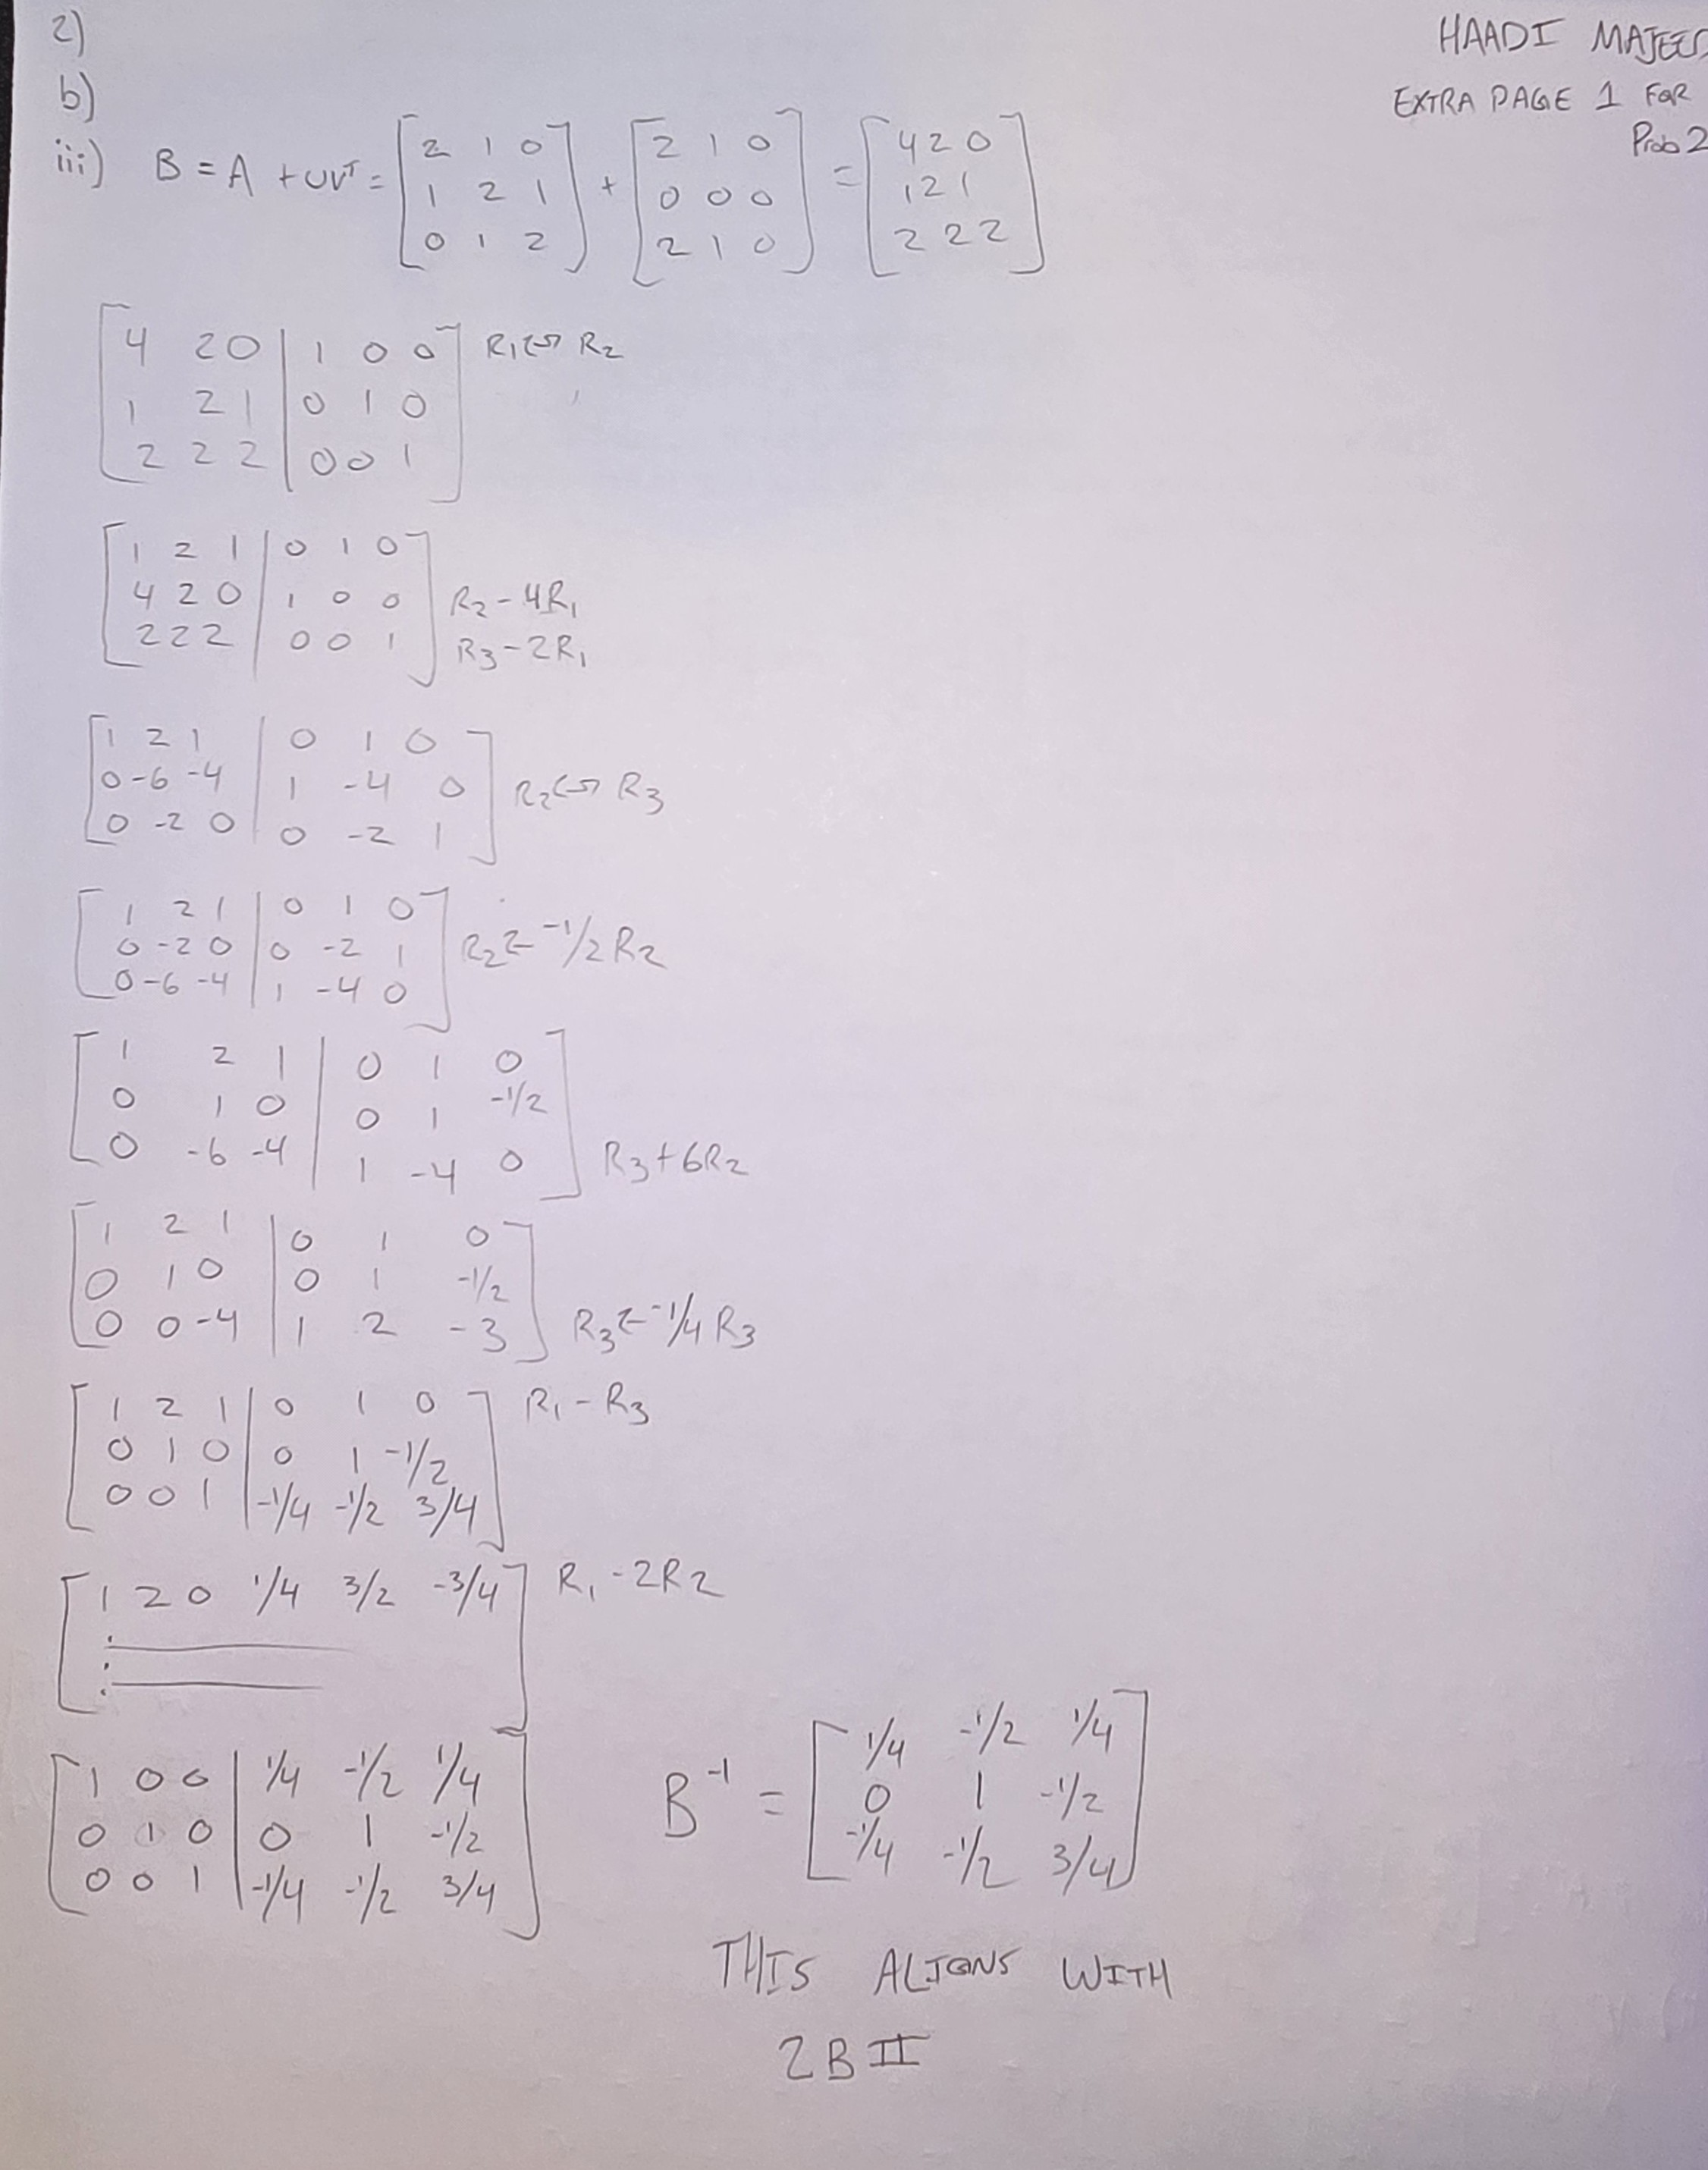
\includegraphics[width=\paperwidth,height=\paperheight,keepaspectratio,angle=0]{page5.jpg}
\end{figure}

\clearpage

\begin{figure}[p]
  \centering
  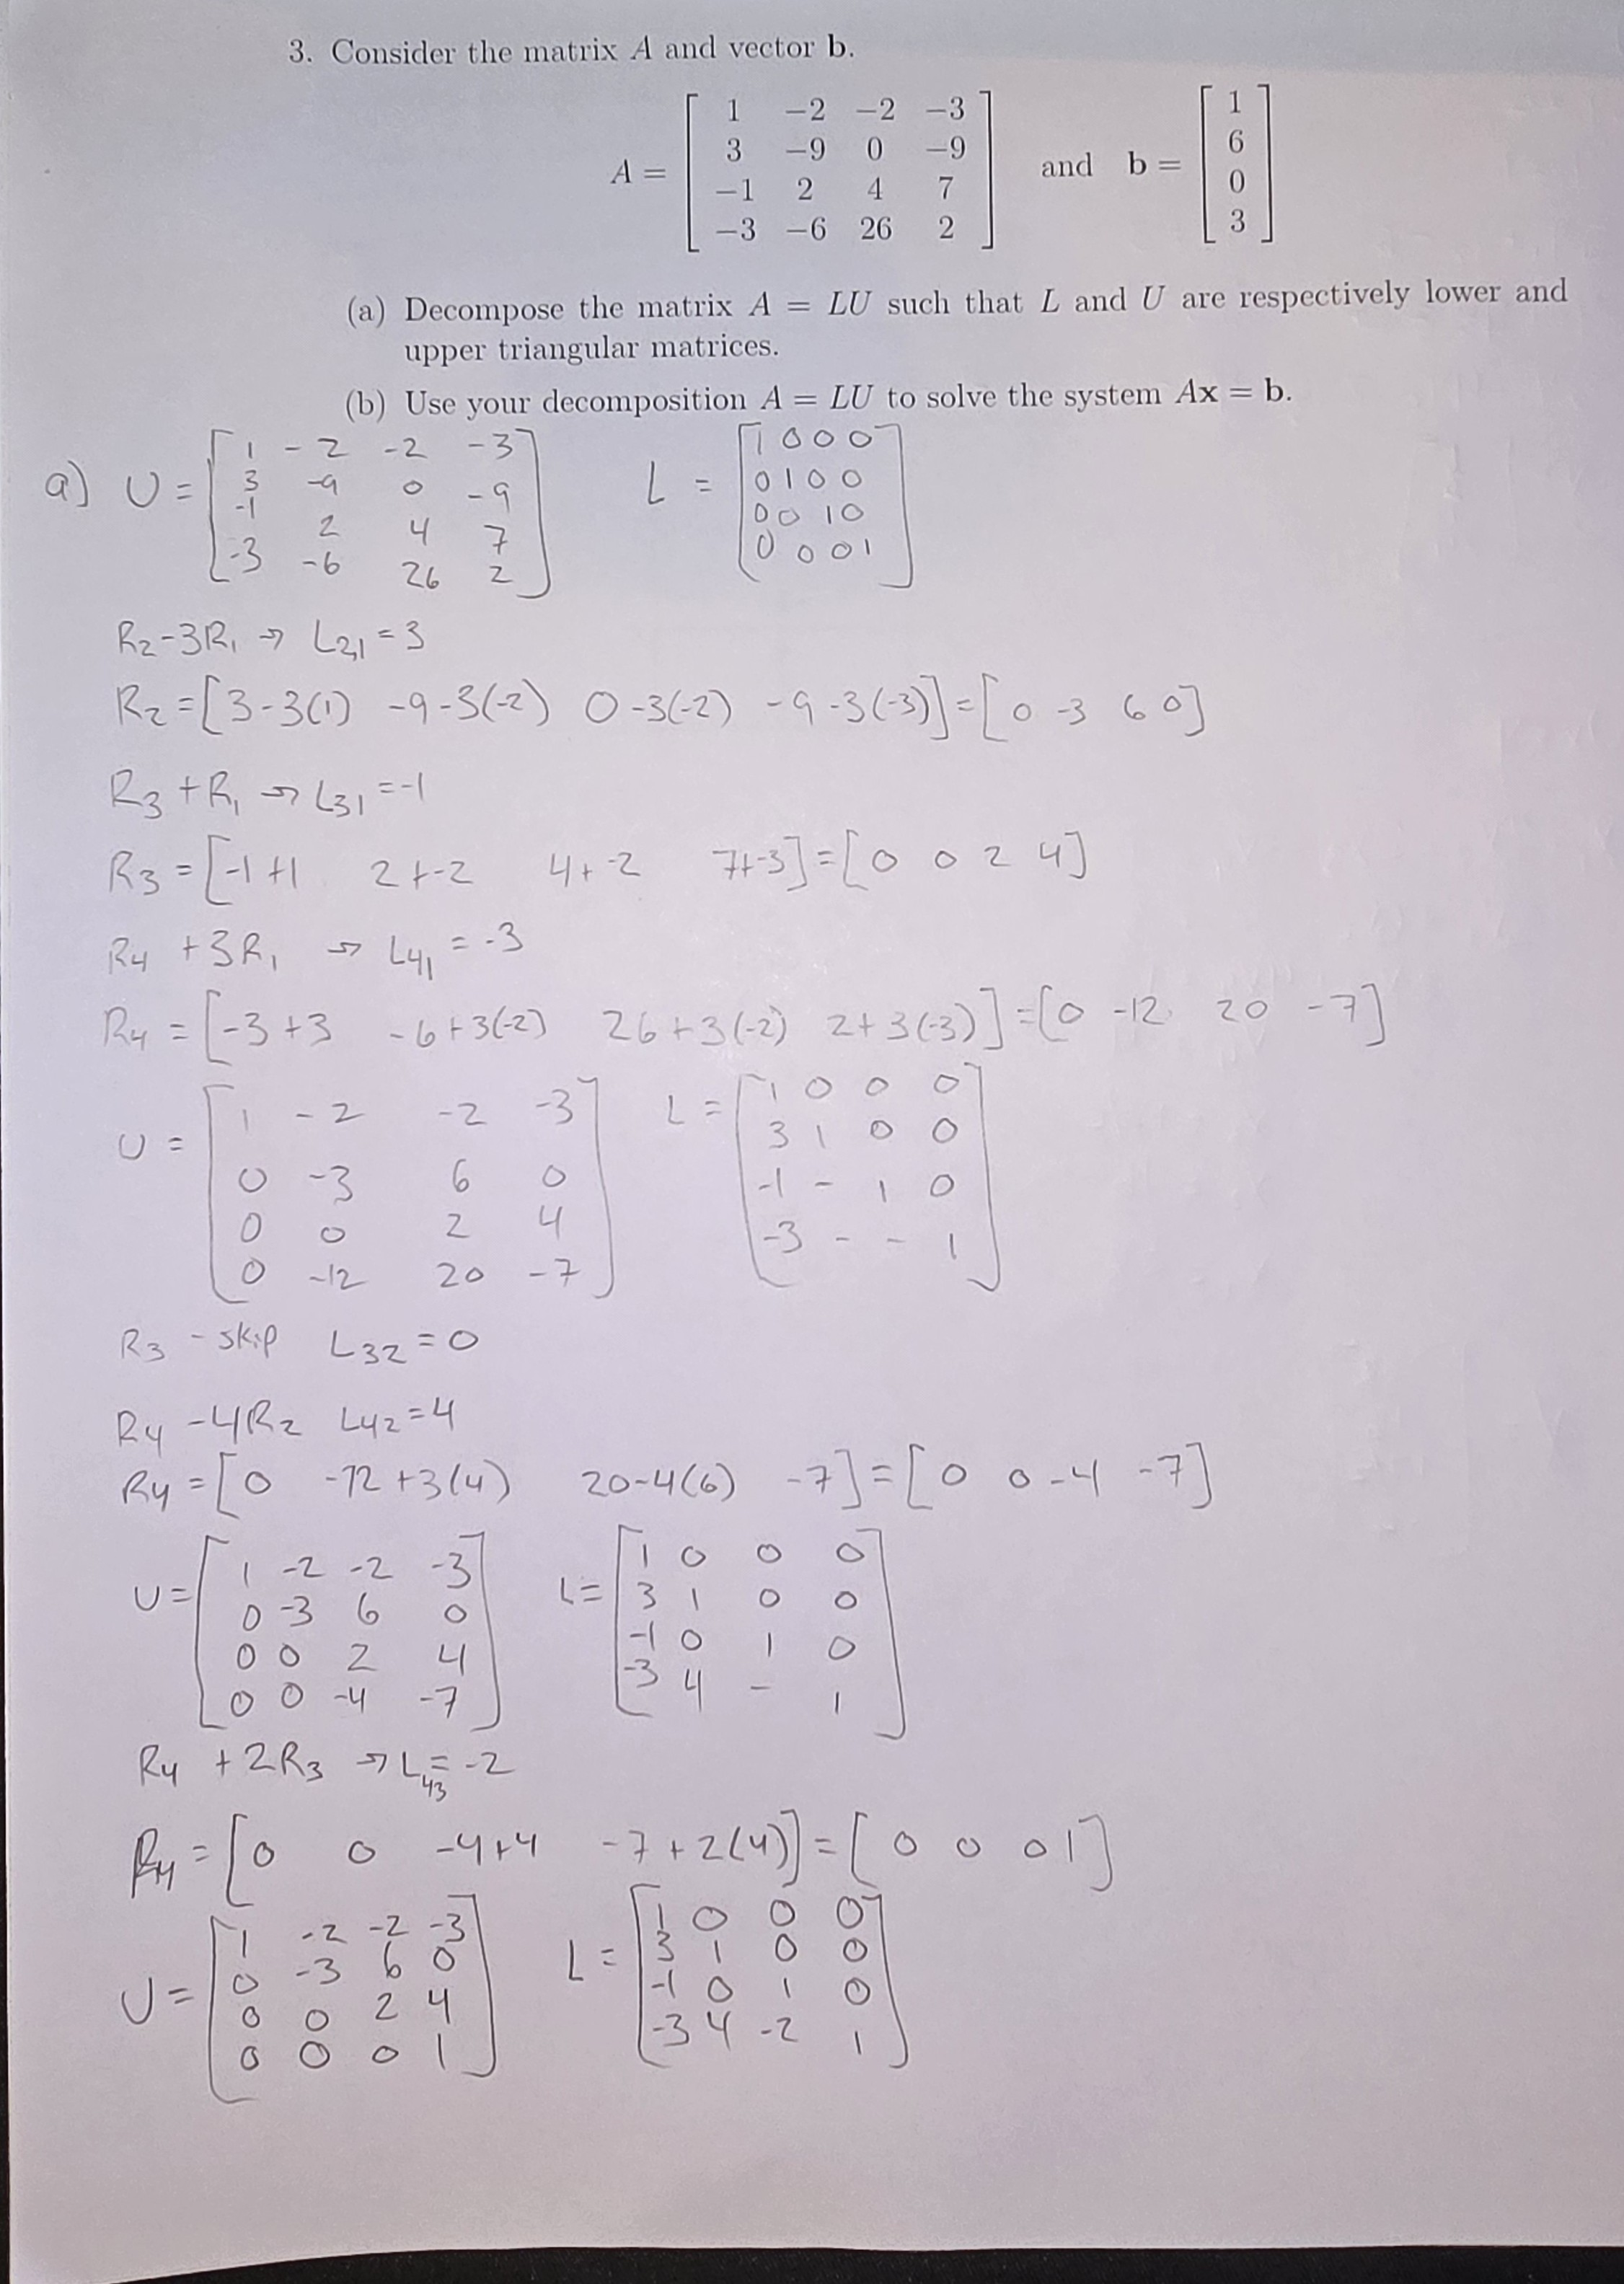
\includegraphics[width=\paperwidth,height=\paperheight,keepaspectratio,angle=0]{page6.jpg}
\end{figure}

\clearpage

\begin{figure}[p]
  \centering
  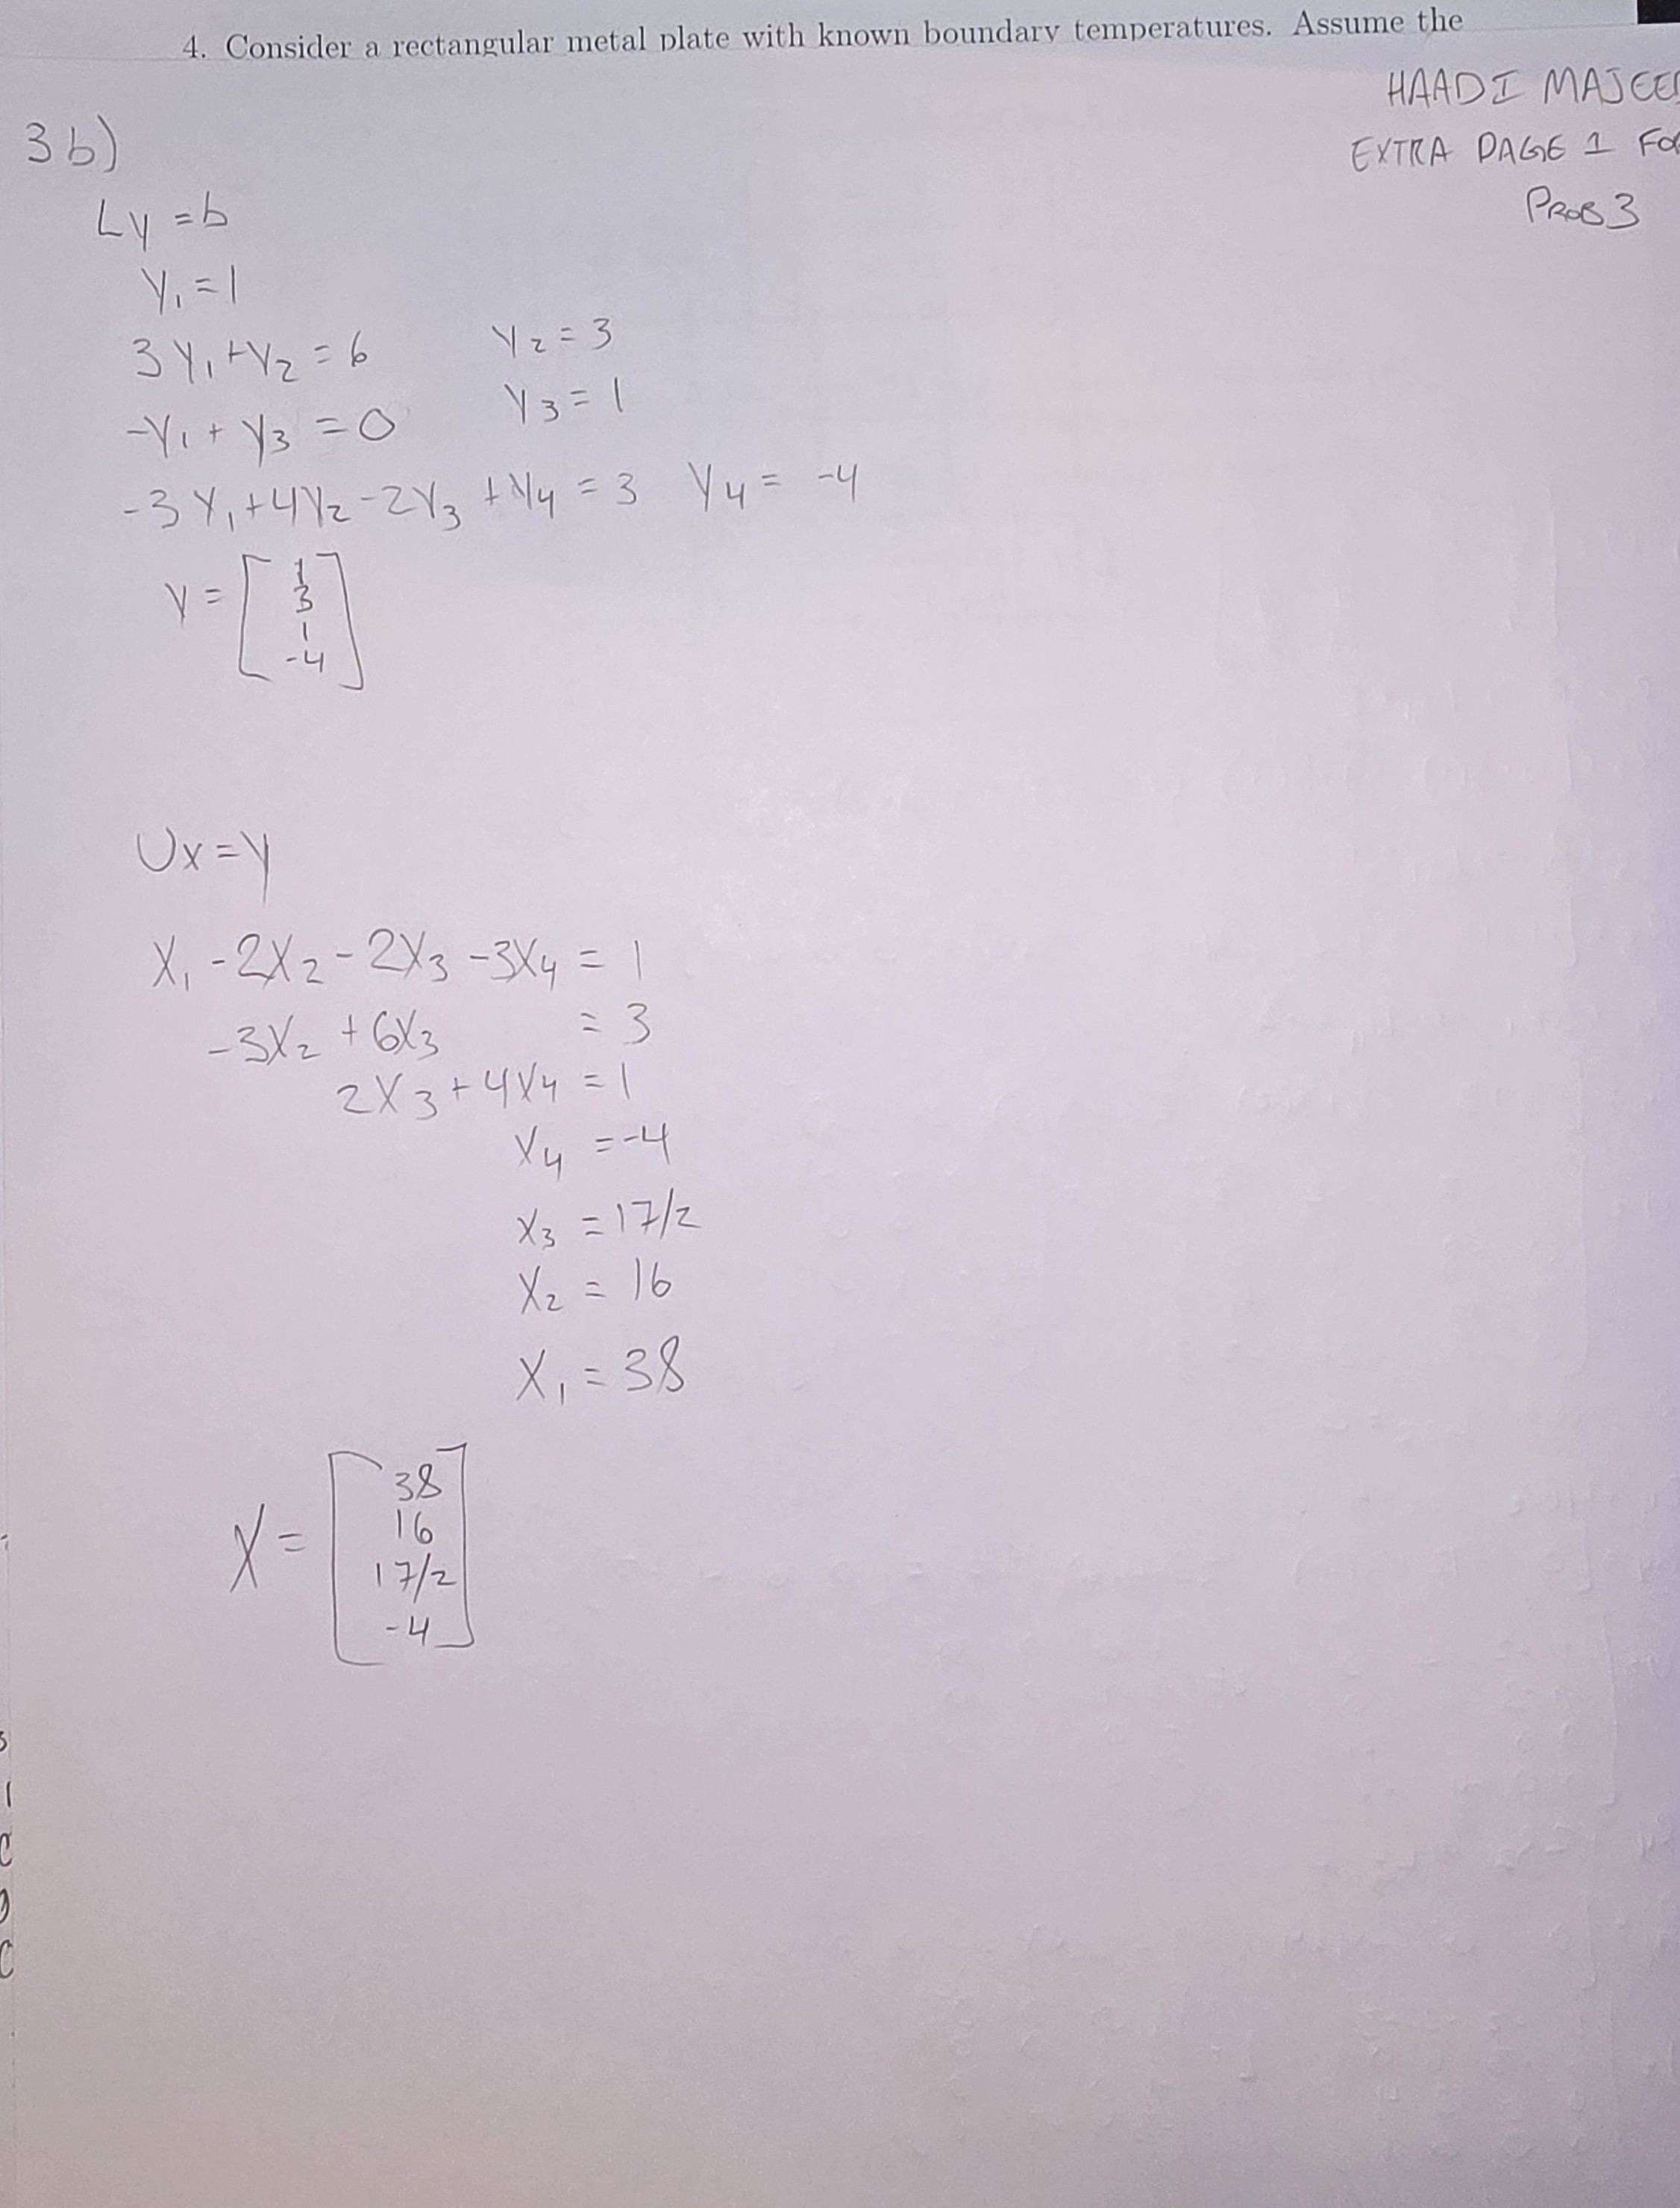
\includegraphics[width=\paperwidth,height=\paperheight,keepaspectratio,angle=0]{page7.jpg}
\end{figure}

\clearpage

\begin{figure}[p]
  \centering
  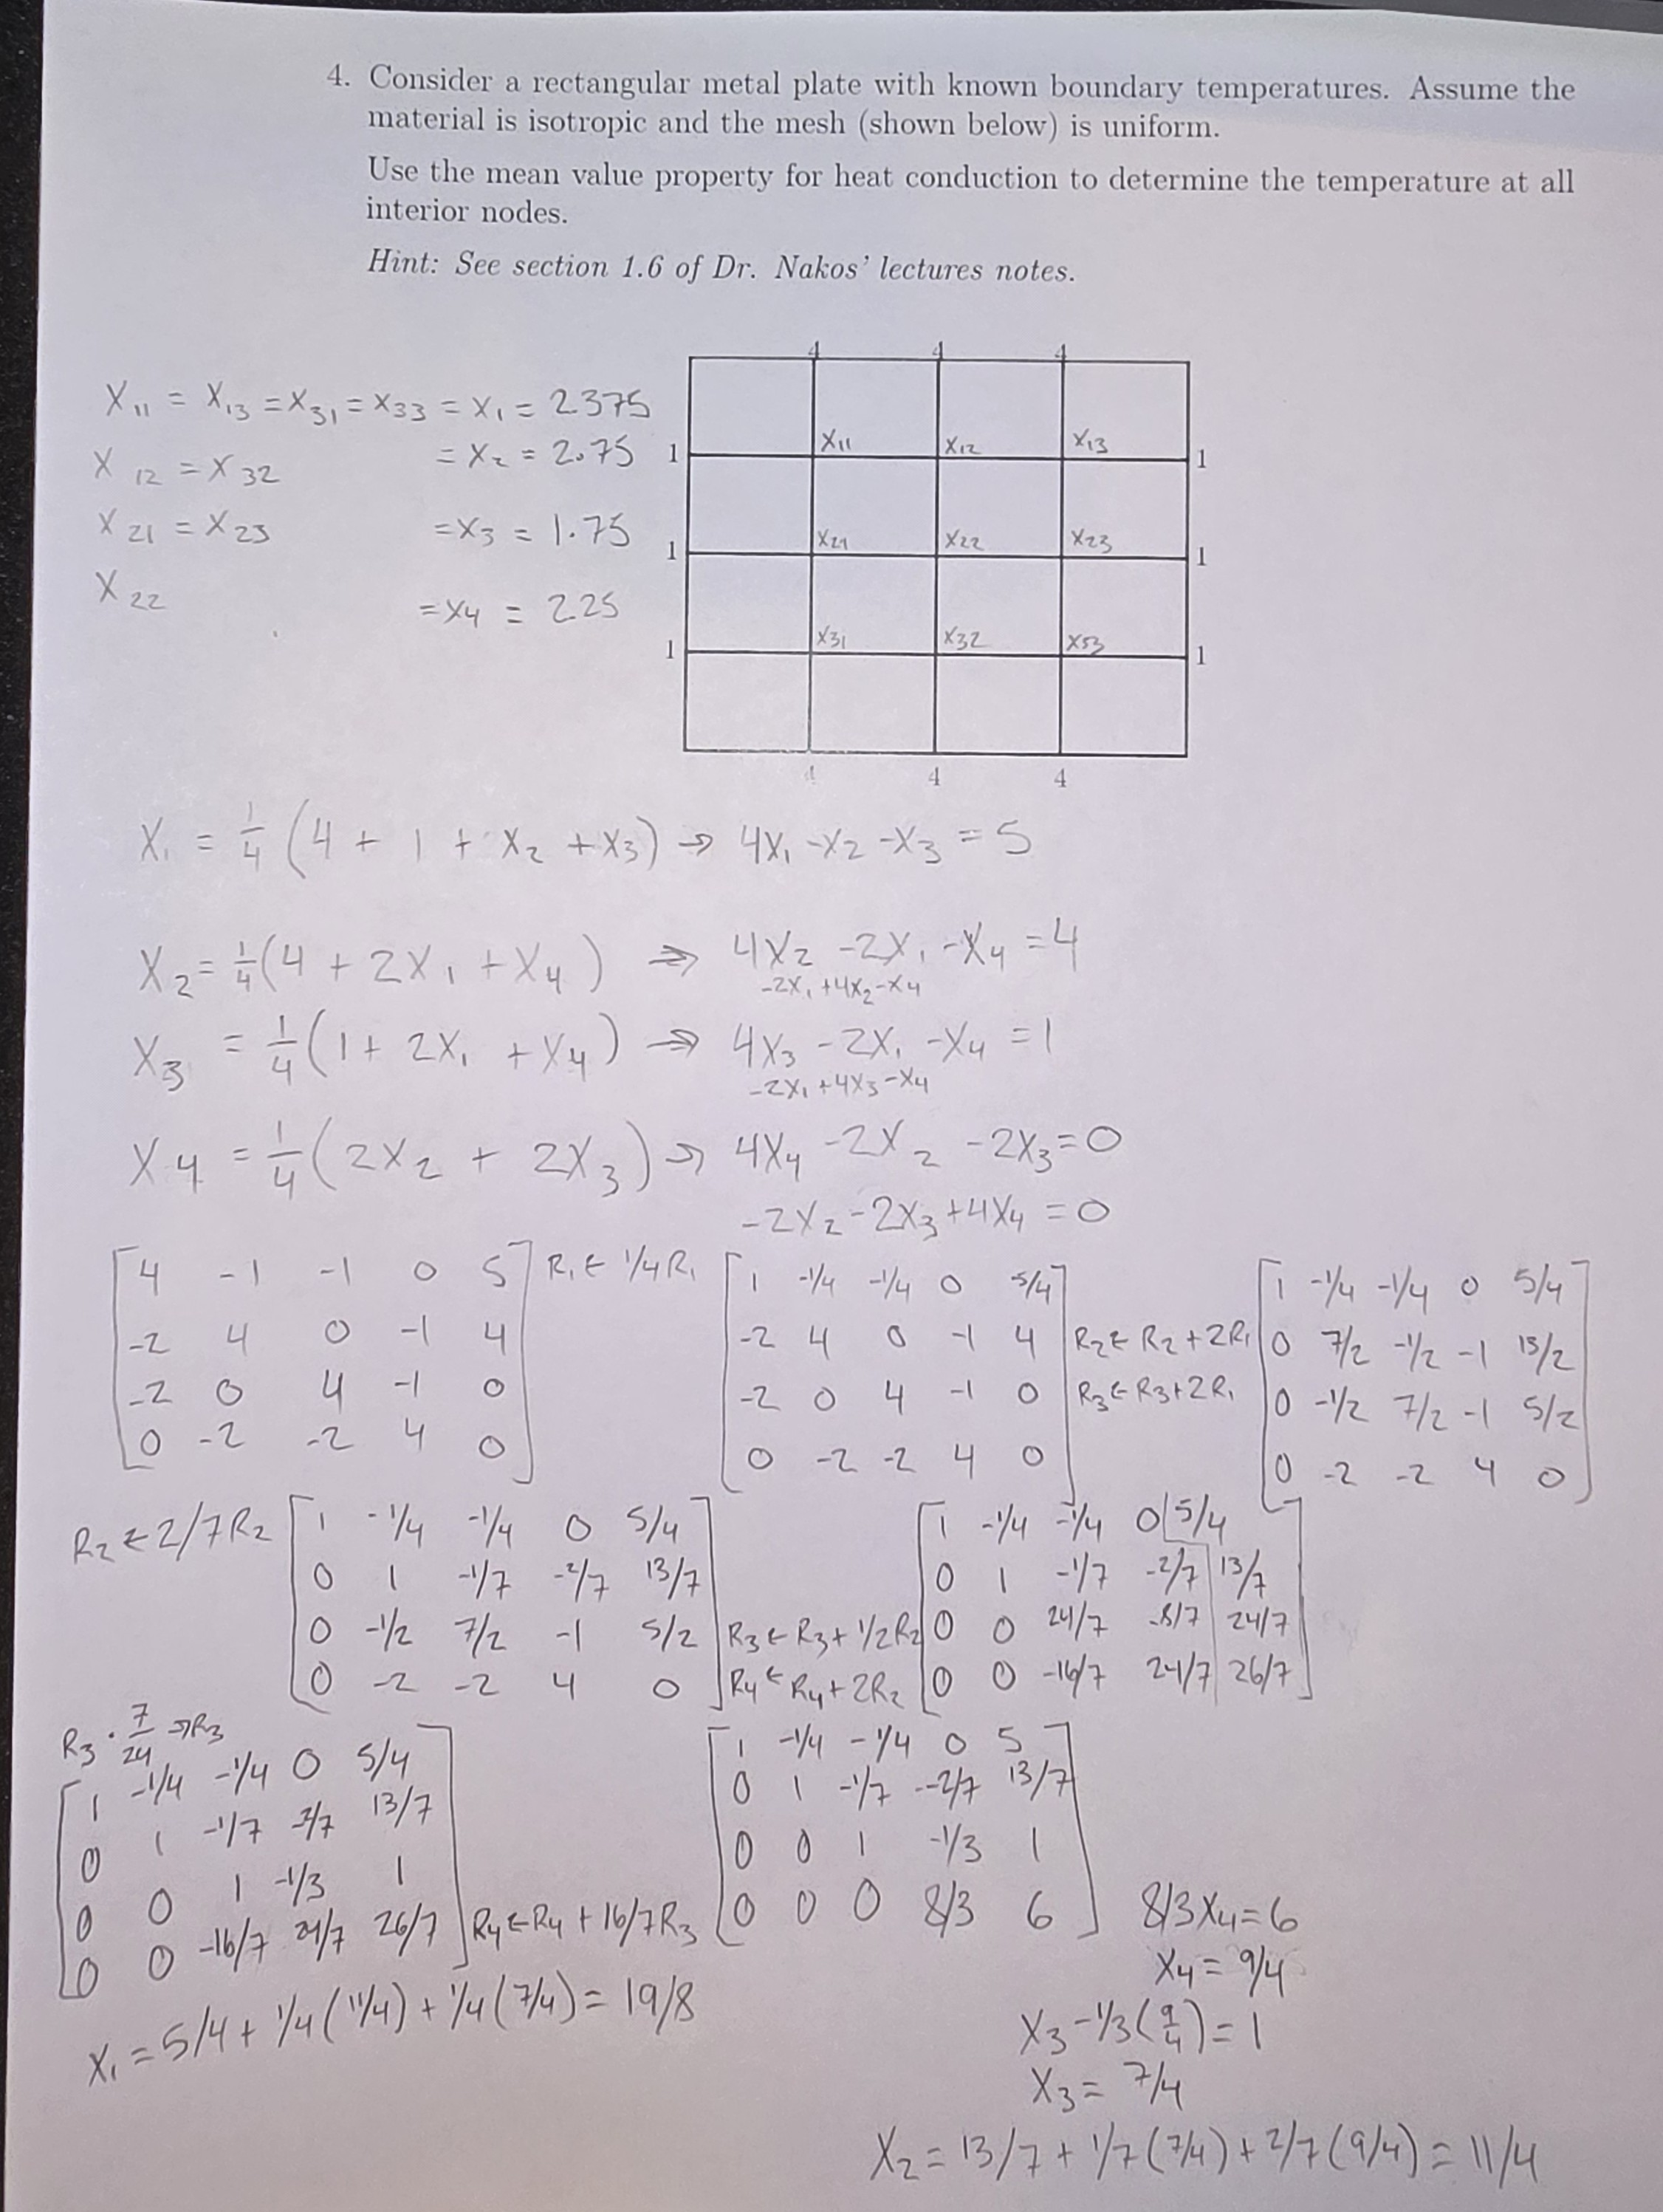
\includegraphics[width=\paperwidth,height=\paperheight,keepaspectratio,angle=0]{page8.jpg}
\end{figure}

\end{document}